\subsection{Three Tier Model}
\label{three_tier_model_section}

In section \ref{two_tier_model_section}, a typical Two-Tier-Architecture was shown.
But to provide a more comfortable structure, there is the necessity of a Three-
or Multi-Tier-Architecture. If, for example, the location of the database server
was changed then, in a Two-Tier-Architecture, all clients would have to be updated.
Figure \ref{three_tier_architecture_figure} makes a proposition to solve this problem.

\begin{figure}[ht]
    \begin{center}
       \includegraphics[scale=0.45]{images/three_tier_architecture.eps}
       \caption{Three-Tier-Architecture}
       \label{three_tier_architecture_figure}
    \end{center}
\end{figure}
